\begin{figure}
    \begin{enumerate}
        \item[(a)] 
\includegraphics[scale=1.02]{plot_rank_similarity_papertop.pdf}\\
        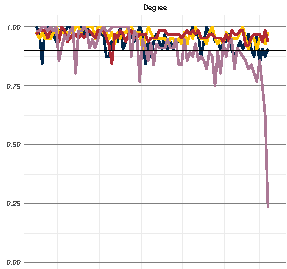
\includegraphics[scale=1.02]{plot_rank_similarity_paper_degree.pdf}\hspace*{0.1mm}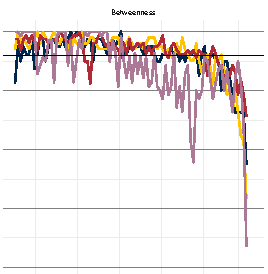
\includegraphics[scale=1.02]{plot_rank_similarity_paper_betweenness.pdf}\hspace*{-0.4mm}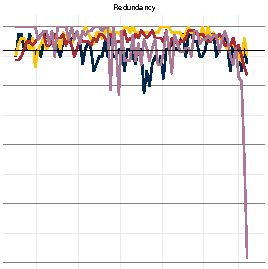
\includegraphics[scale=1.02]{plot_rank_similarity_paper_redundancy.pdf}\\
        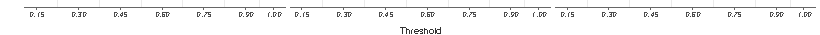
\includegraphics[scale=1.02]{plot_rank_similarity_paperbottom.pdf}
        \vspace*{-0.6cm}
        \item[(b)] \hspace*{-0.25cm}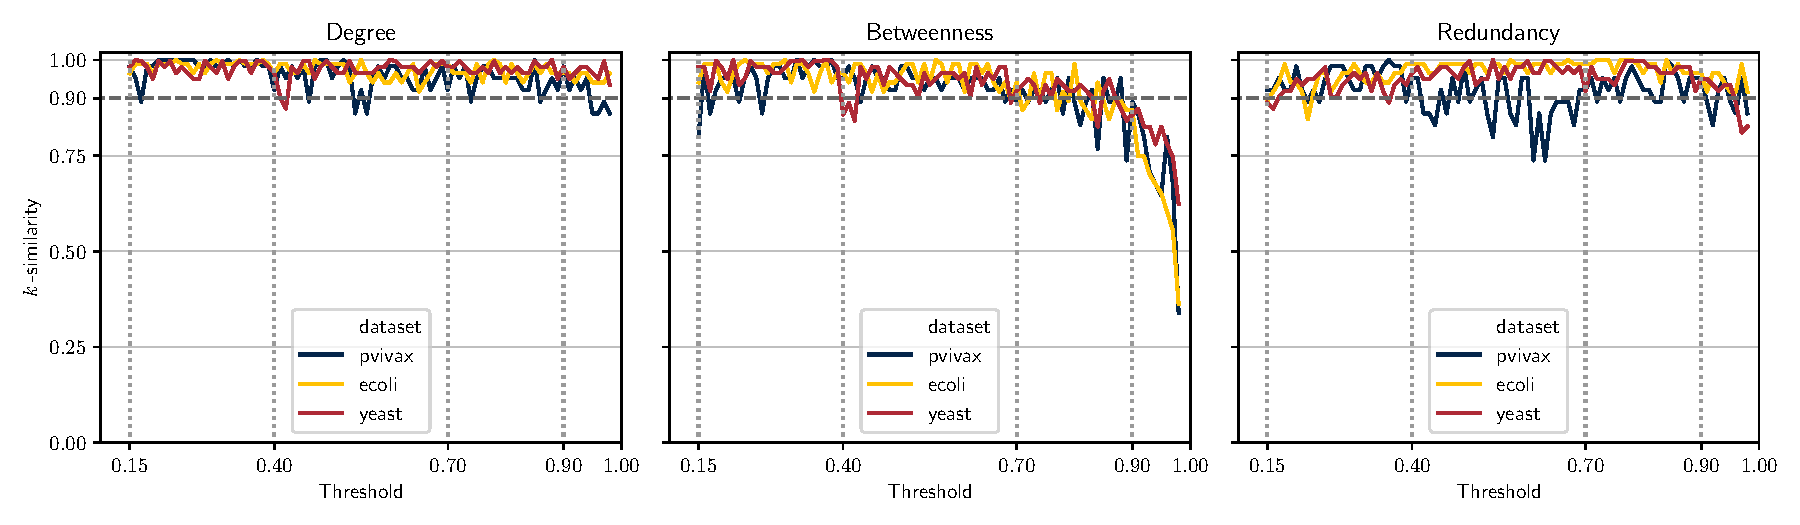
\includegraphics[align=t,width=0.97\linewidth]{plot_rank_similarity_graffs.pdf}
    \end{enumerate}
    \vspace*{-0.6cm}
    \caption{$k$-similarity plots between ranks of graphs derived from protein networks at consecutive thresholds, taking results from The Paper~(a) and \graffs~(b).
    The $k$ coefficient was set to $0.01$ for computing these plots.}
    \label{fig:plot_rank_similarity}
    %\footnotetext{Chosen according to \url{https://github.com/lbozhilova/measuring_rank_robustness/blob/master/figure_generation.R#L28}}
\end{figure}
